\section{Teilversuch 5: Fraunhofer-Beugung an Doppelspalt und Mehrfachspalt}
	Aus zeitlichen Gründen ist dieses Teilversuch für alle von Marlene Schramm durchgeführt. Die Bilder für den Doppelspalt sind von Marlene Schramm aufgenommen und die Bilder für den Mehrfachspalt sind von mir aufgenommen. 
	
	\begin{figure}[H]
		\centering
			\begin{tabular}{llll}
				\multicolumn{4}{l}{Doppelspalt} \\
				\toprule
					$b = \num{0.2}$  & $b = \num{0.1}$ & $b = \num{0.1}$ & $b = \num{0.1}$ \\
					$g = \num{0.25}$ & $g = \num{0.2}$ & $g = \num{0.5}$ & $g = \num{1.0}$ \\
				\midrule
					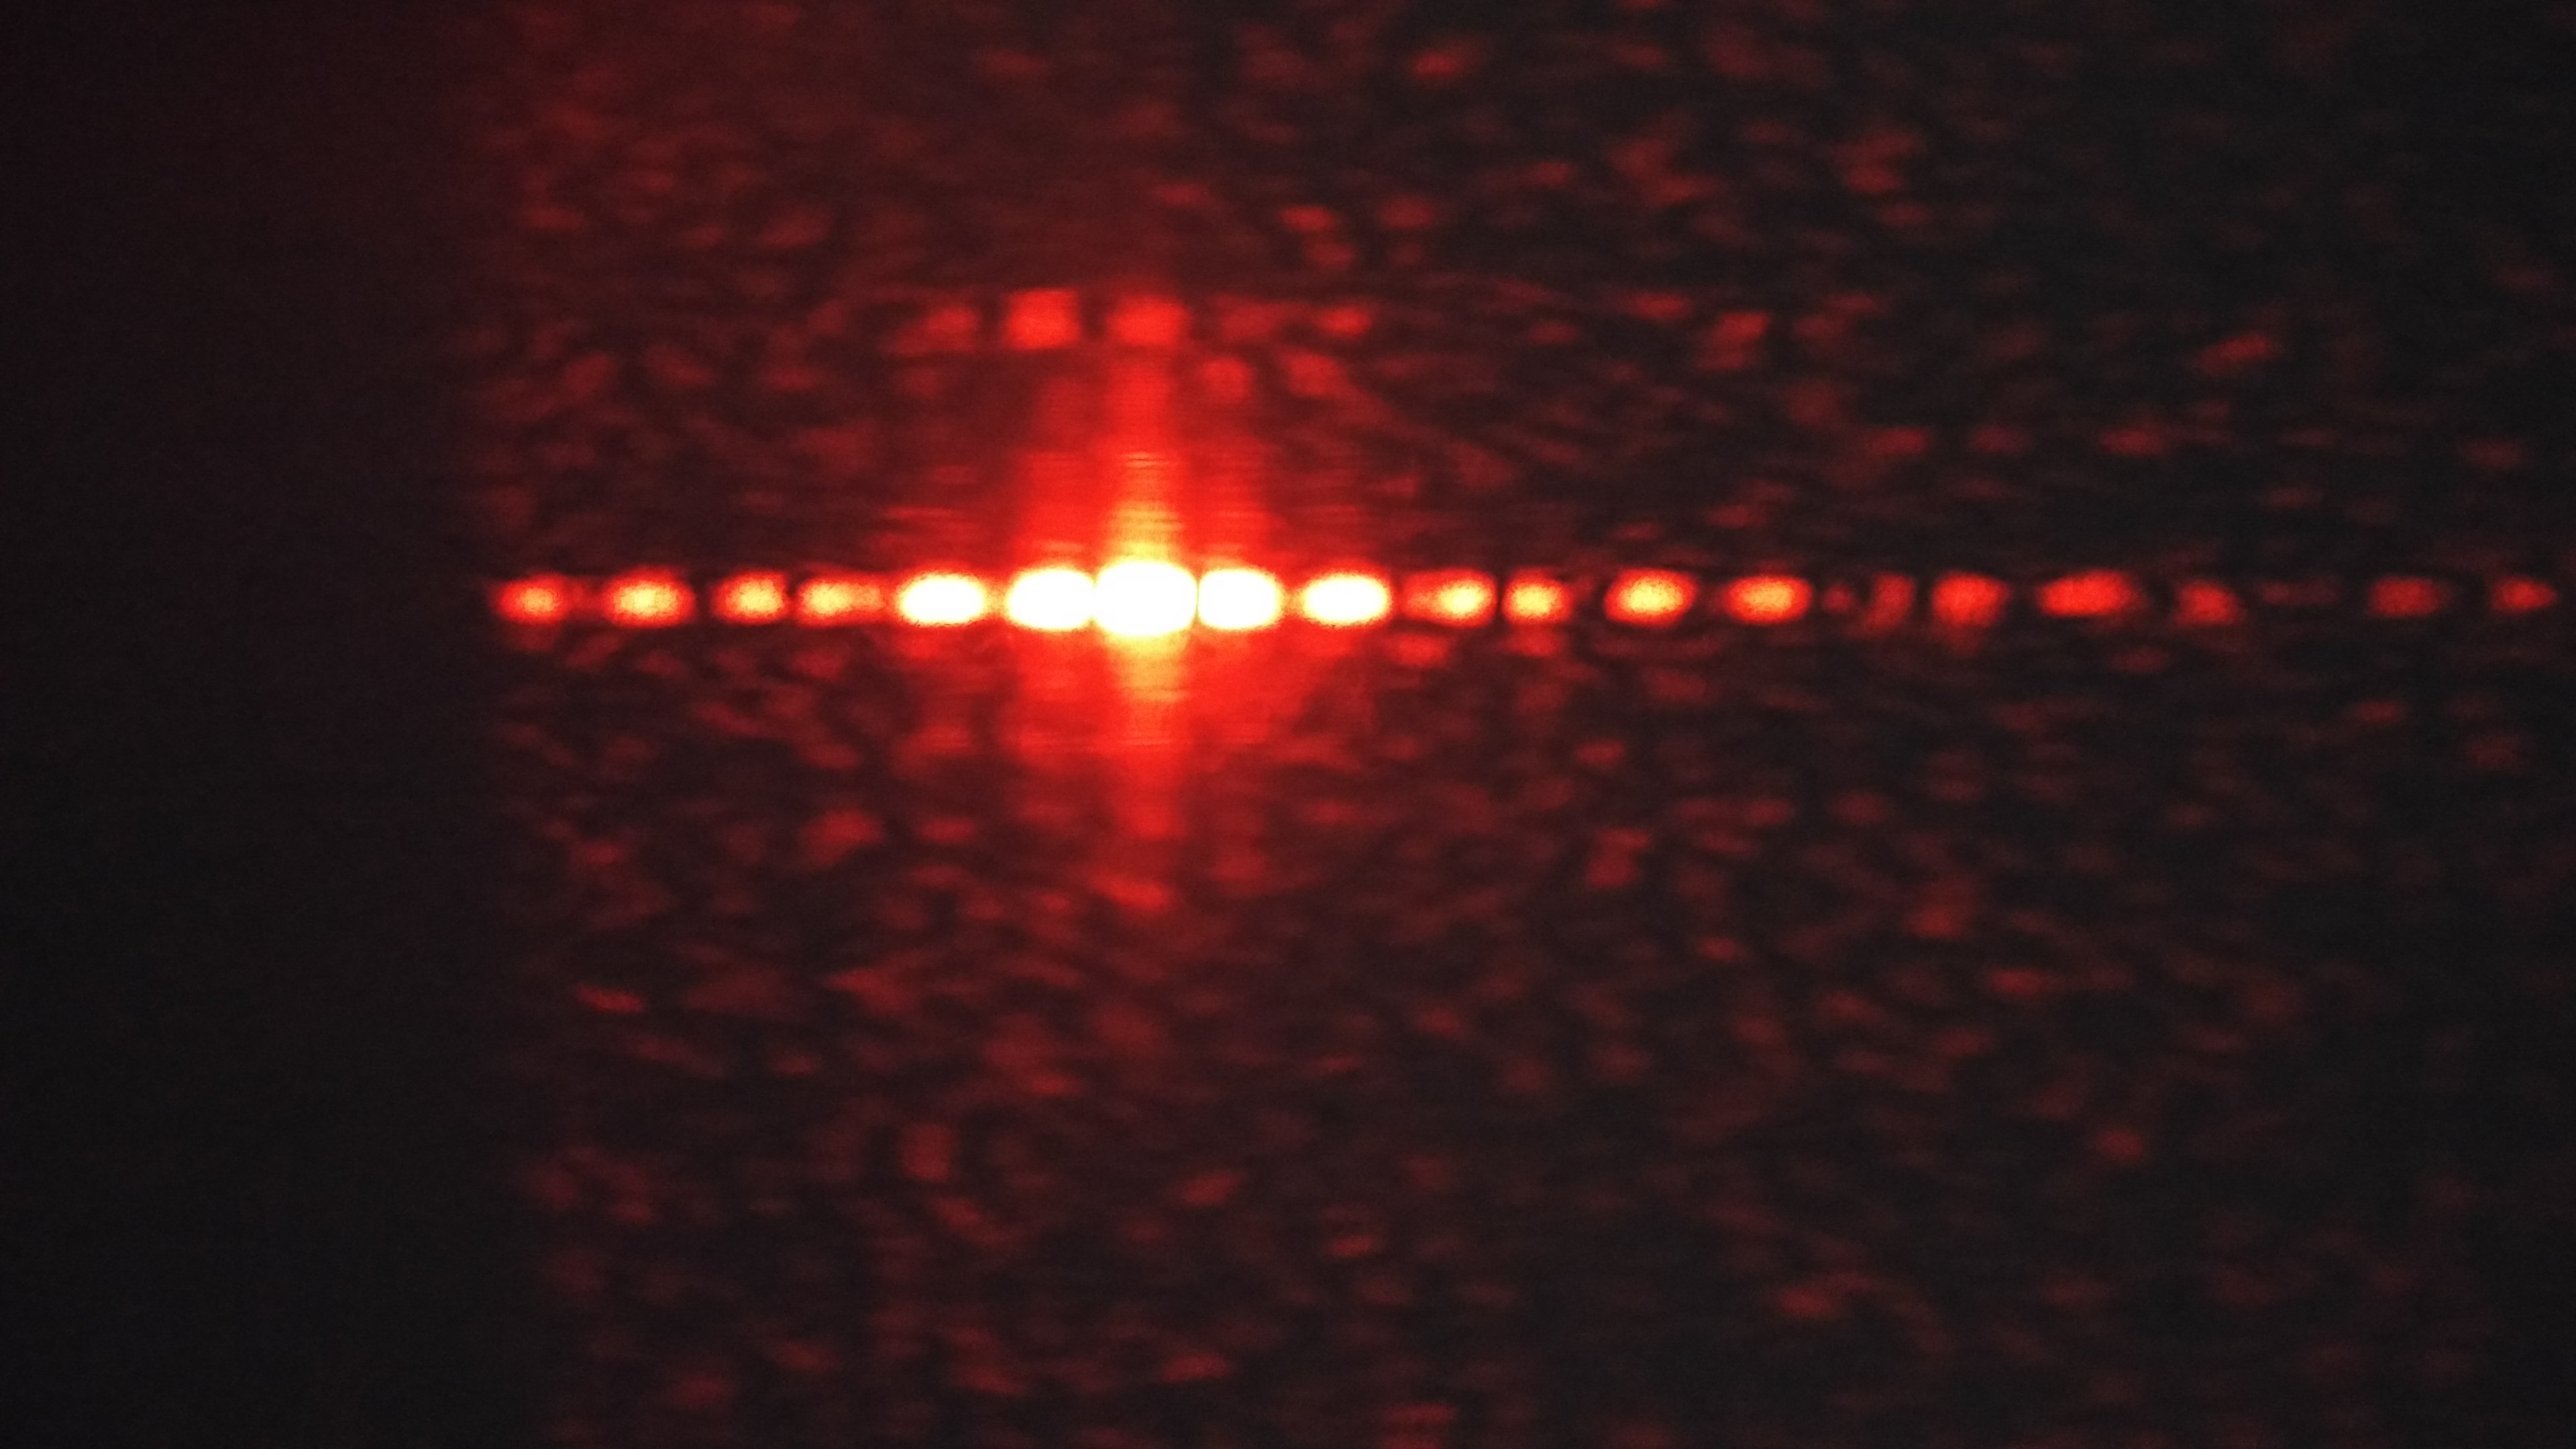
\includegraphics[width=0.22\textwidth]{images/tv5/doppelspalt/b_0.2_g_0.25.jpg} &
					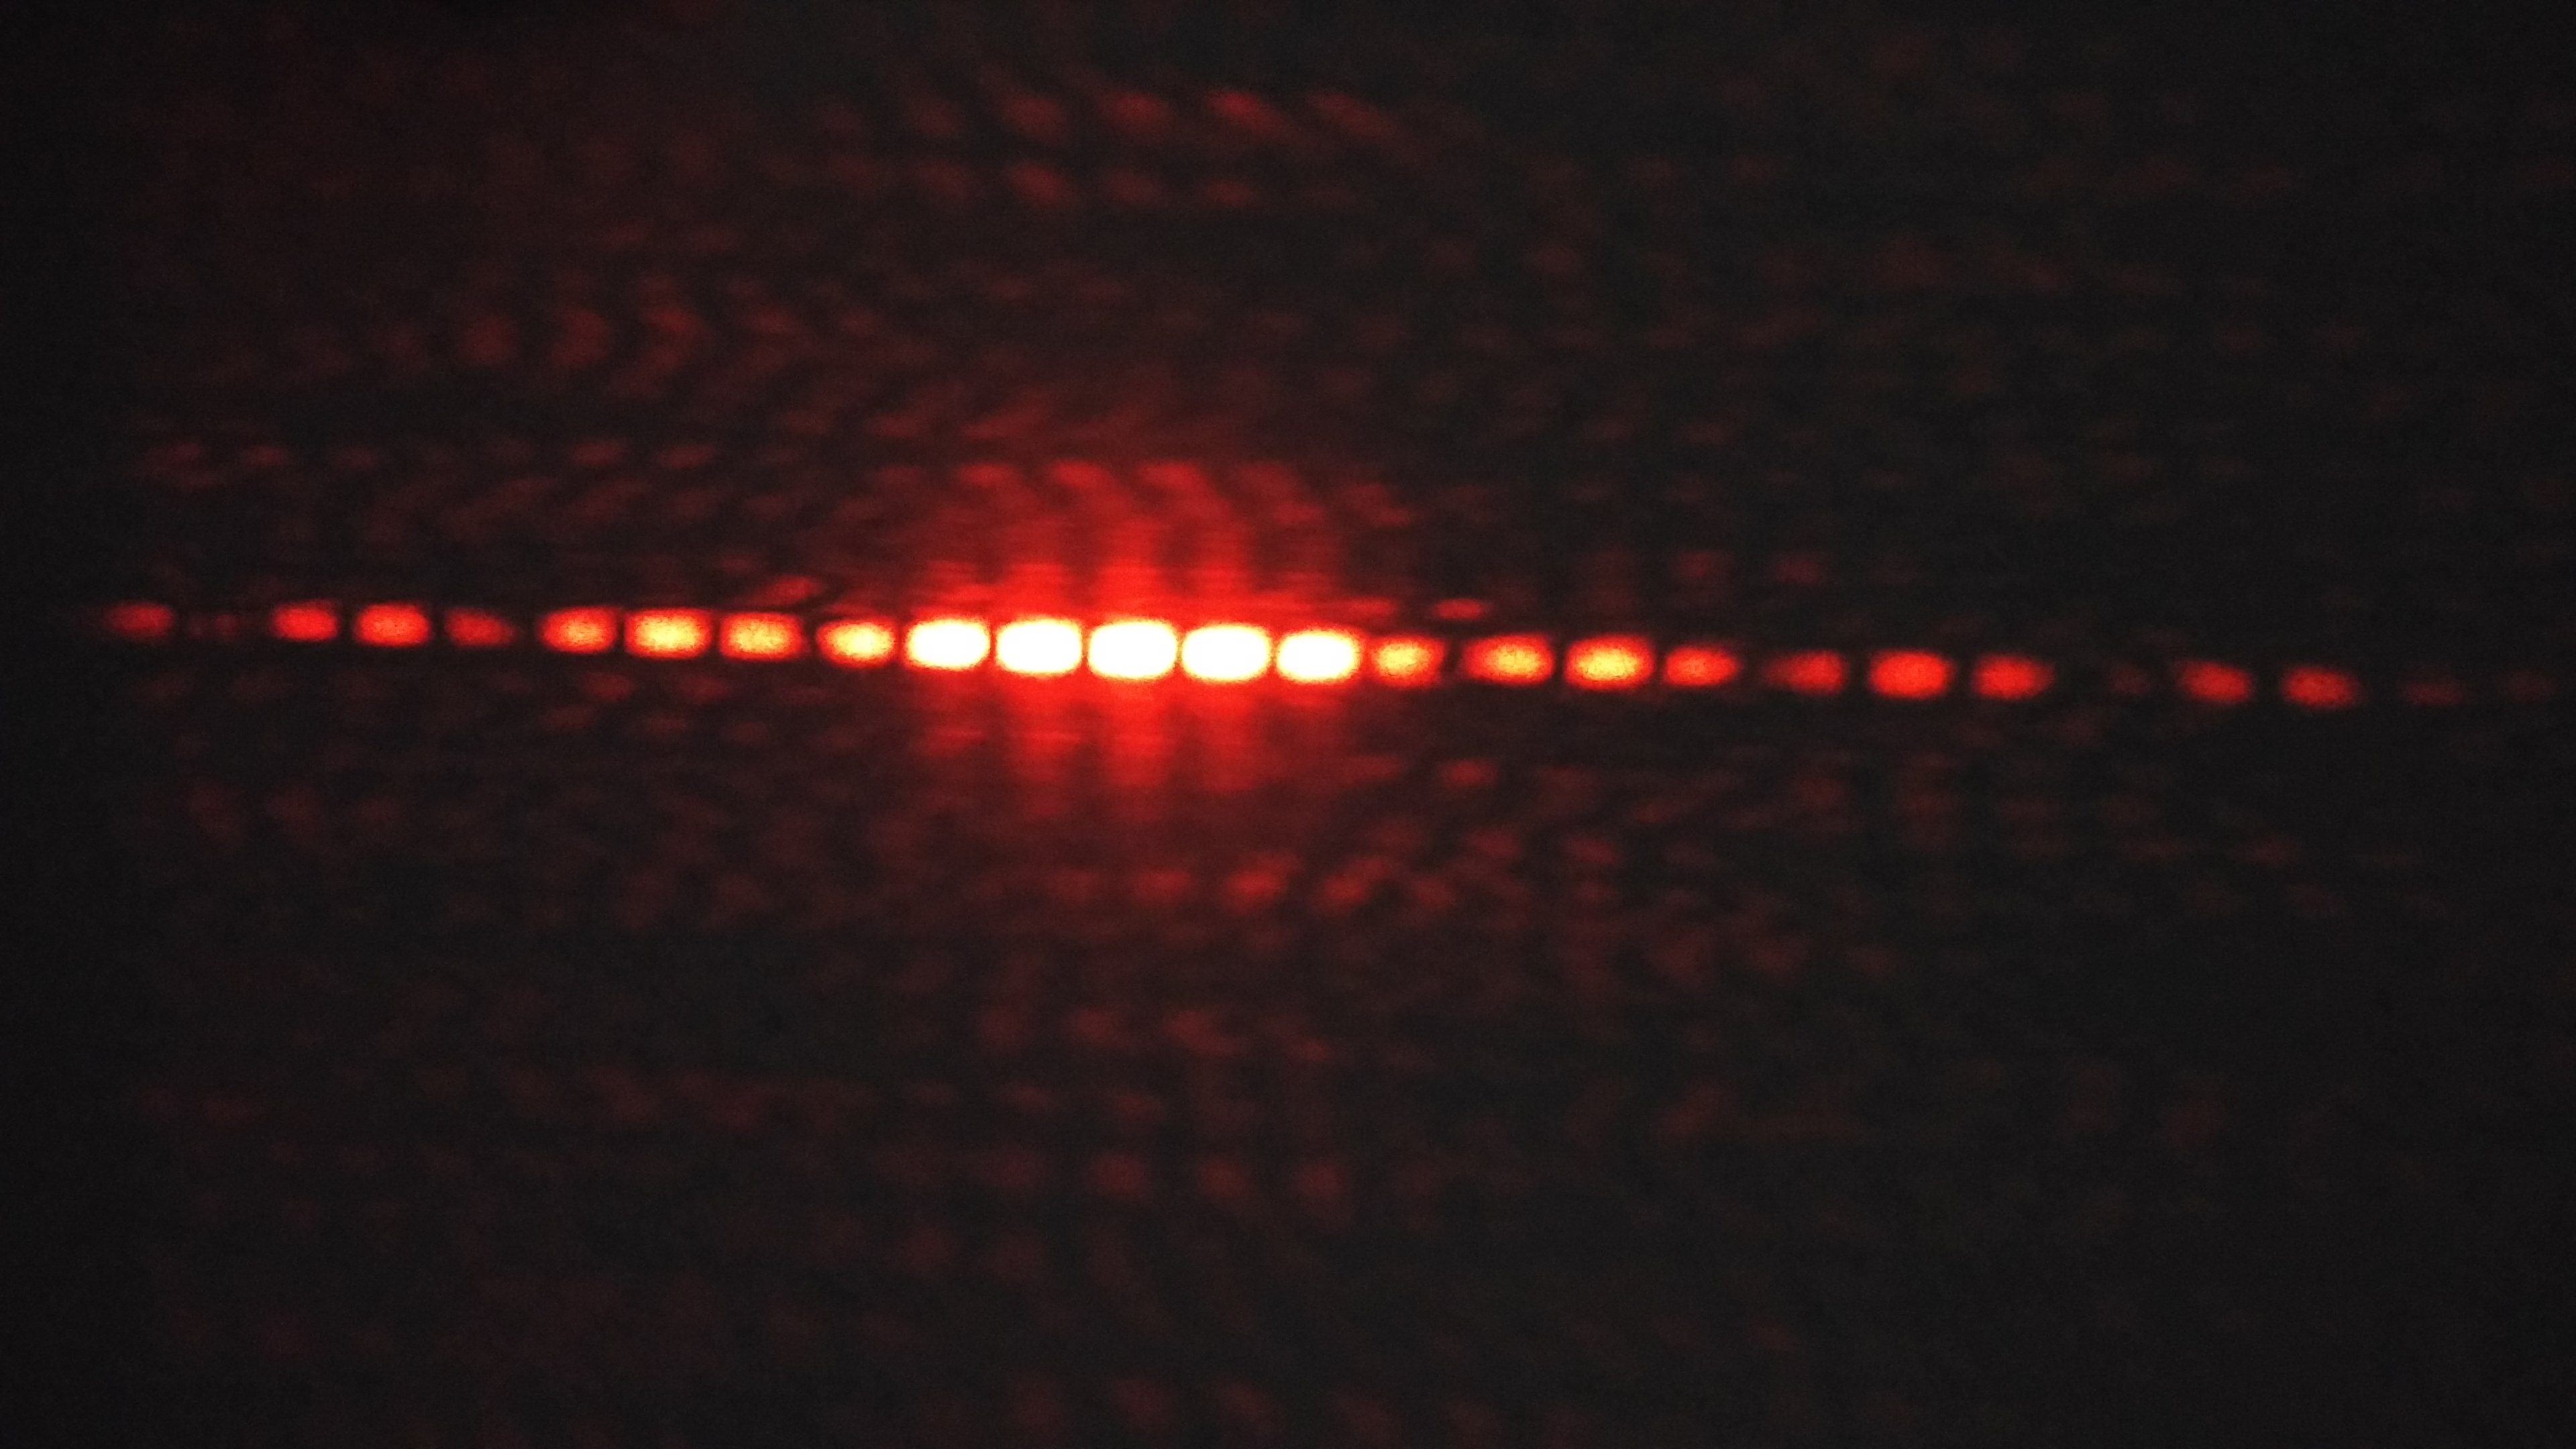
\includegraphics[width=0.22\textwidth]{images/tv5/doppelspalt/b_0.1_g_0.2.jpg} &
					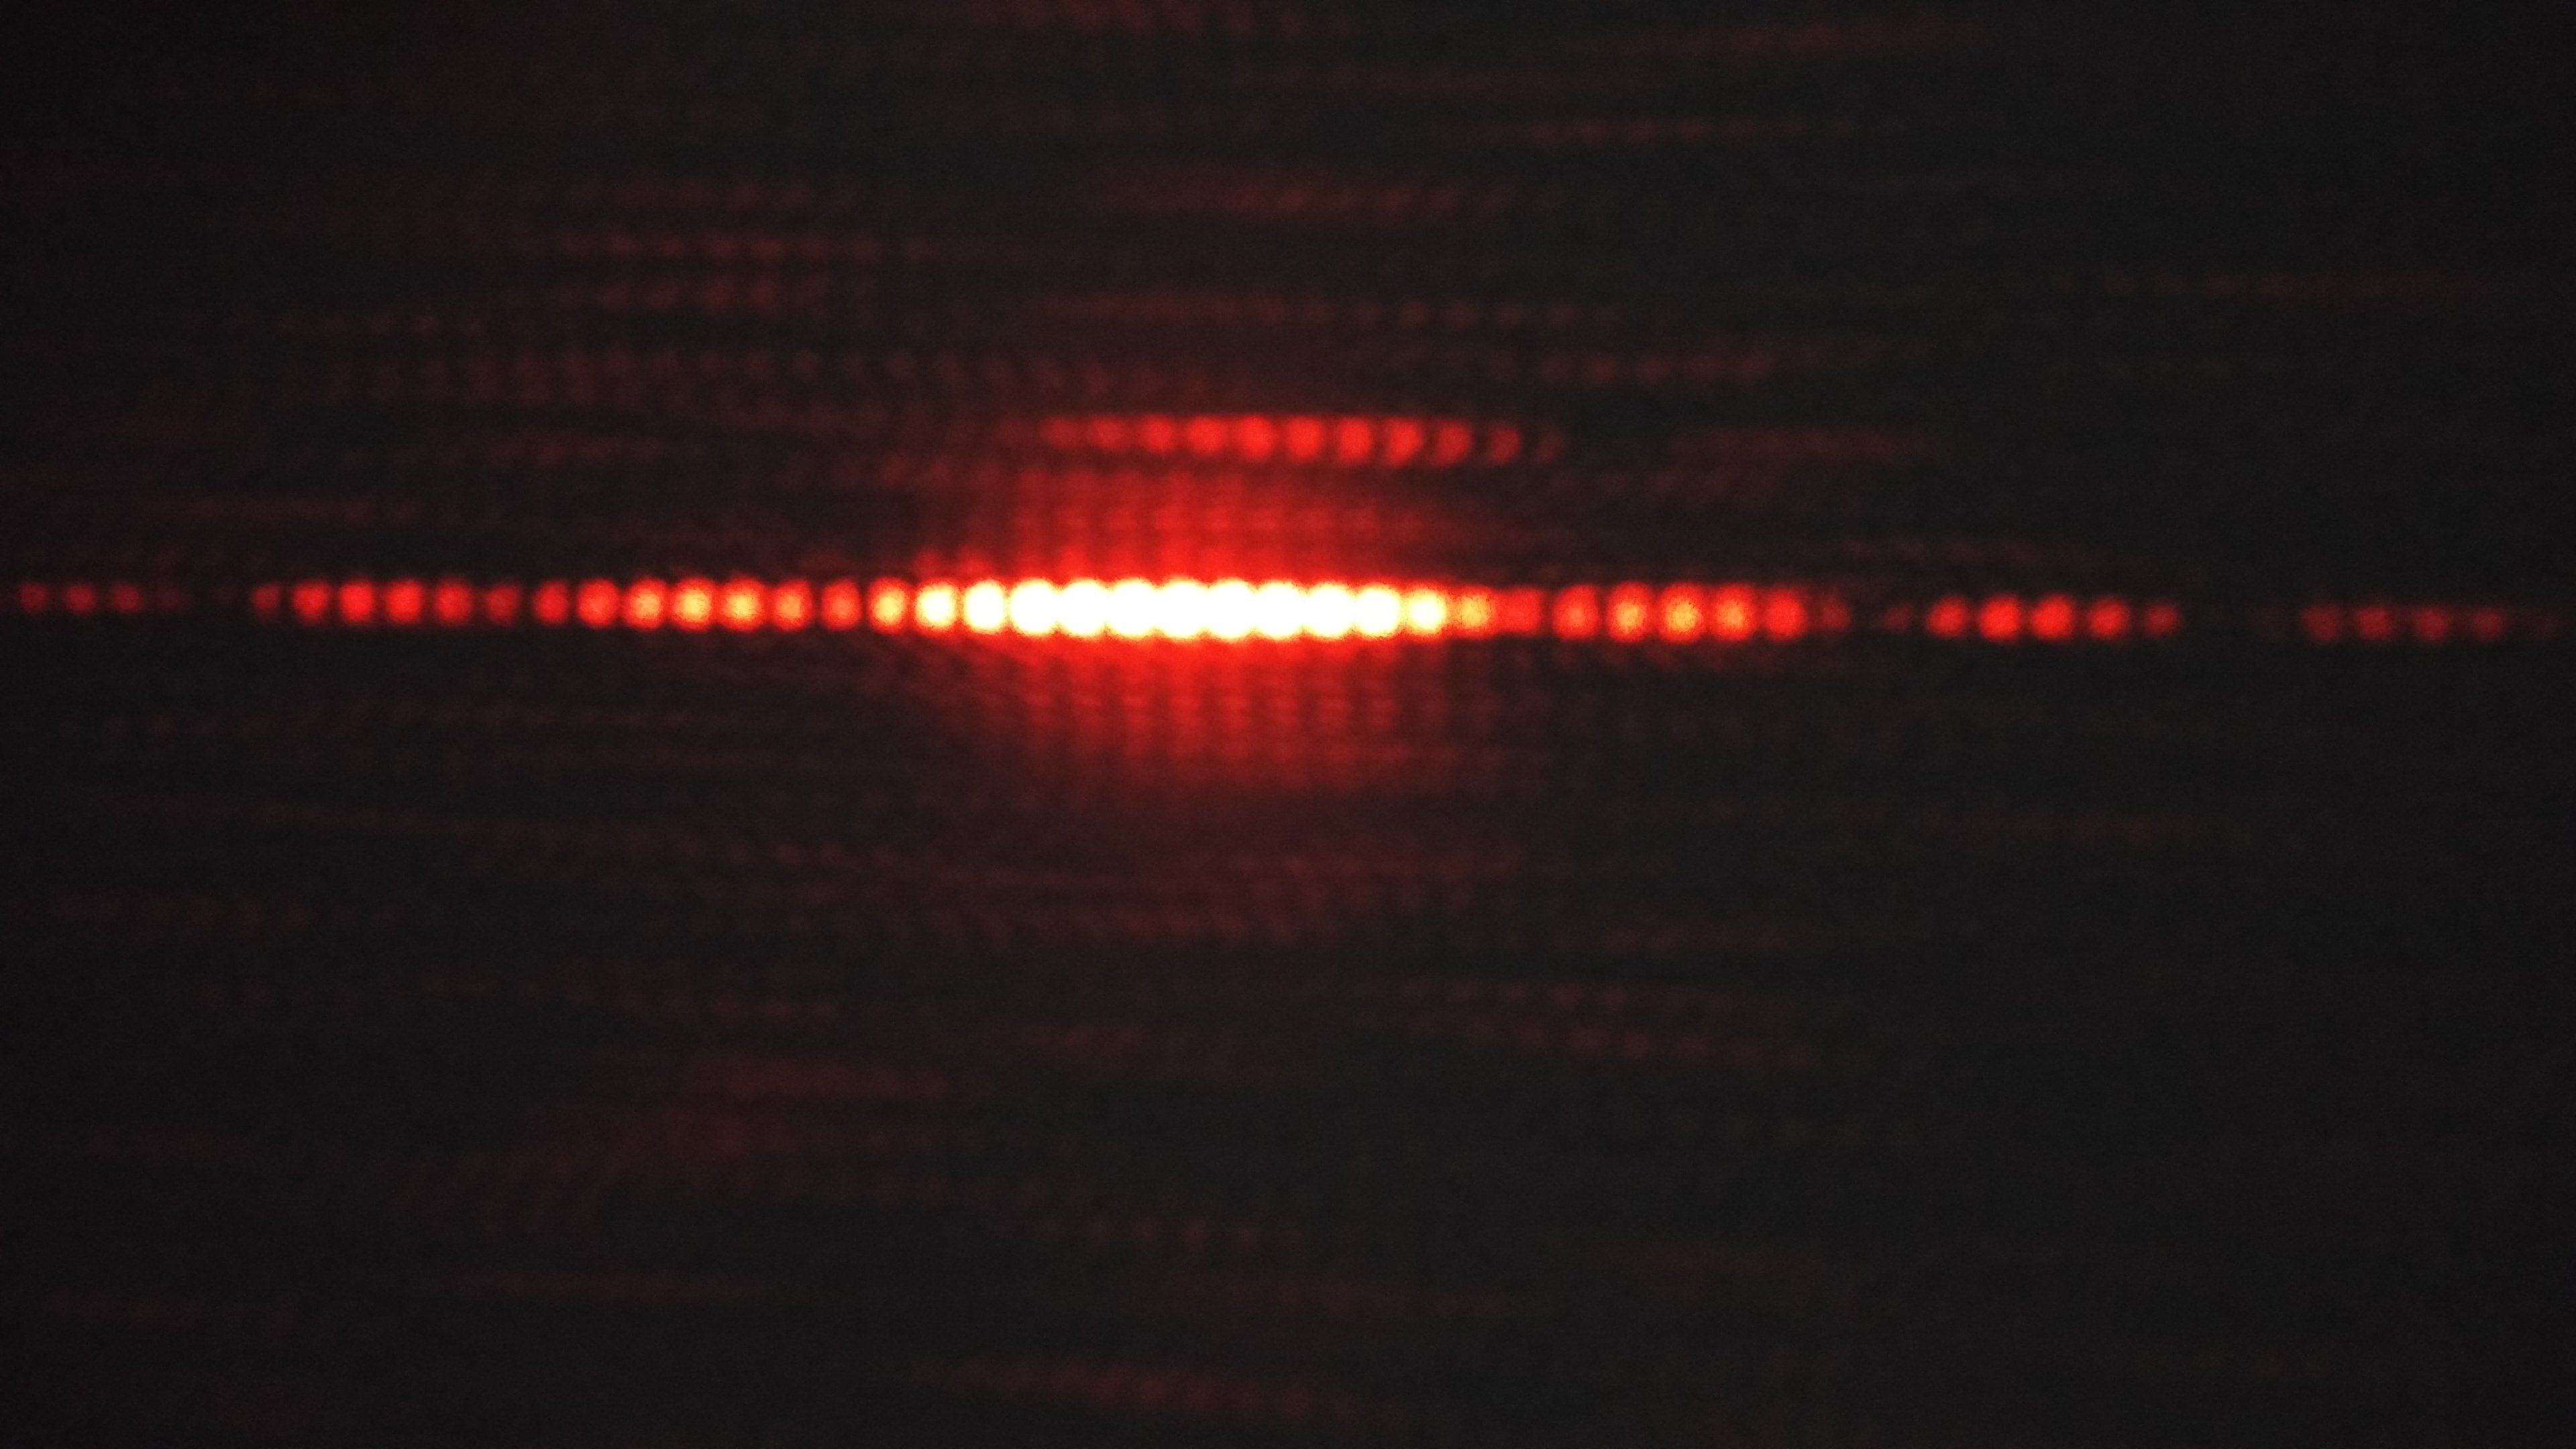
\includegraphics[width=0.22\textwidth]{images/tv5/doppelspalt/b_0.1_g_0.5.jpg} &
					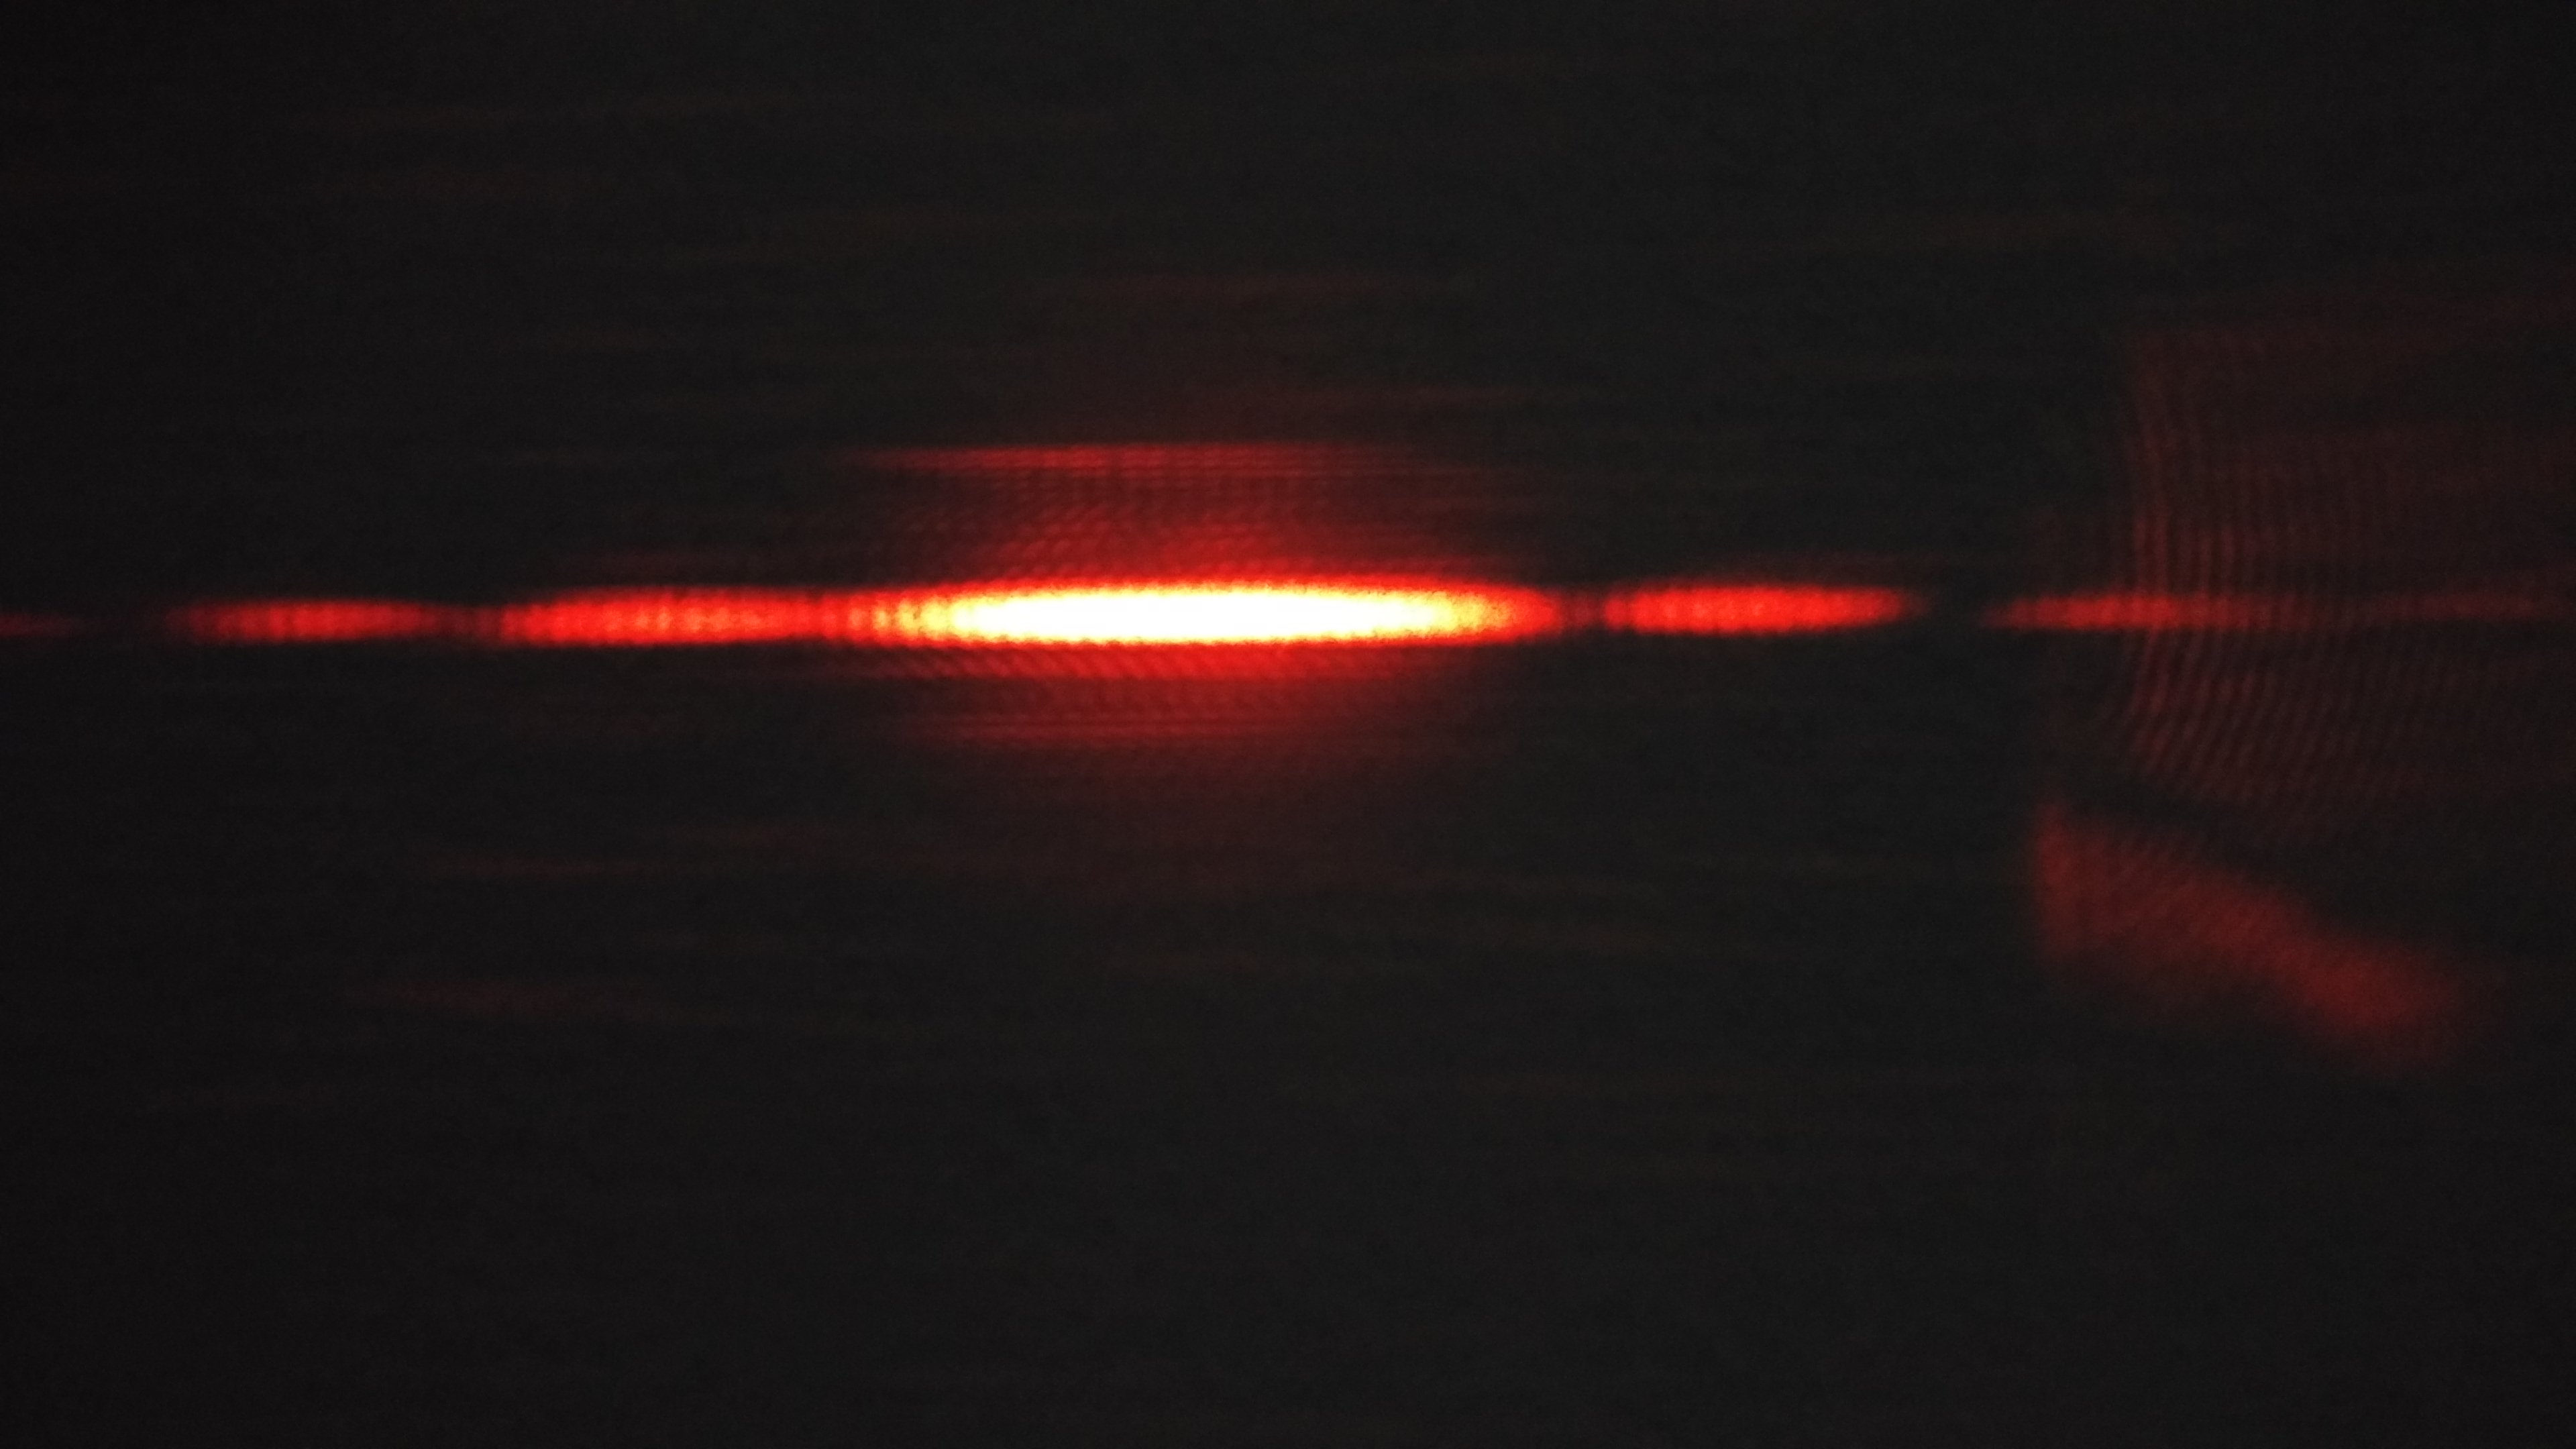
\includegraphics[width=0.22\textwidth]{images/tv5/doppelspalt/b_0.1_g_1.0.jpg} \\
				\bottomrule
				\\
				\multicolumn{4}{l}{Mehrfachspalt ($b = \num{0.1}$, $g = \num{0.25}$)} \\
				\toprule
					$N = 2$ & $N = 3$ & $N = 4$ & $N = 5$ \\
				\midrule
					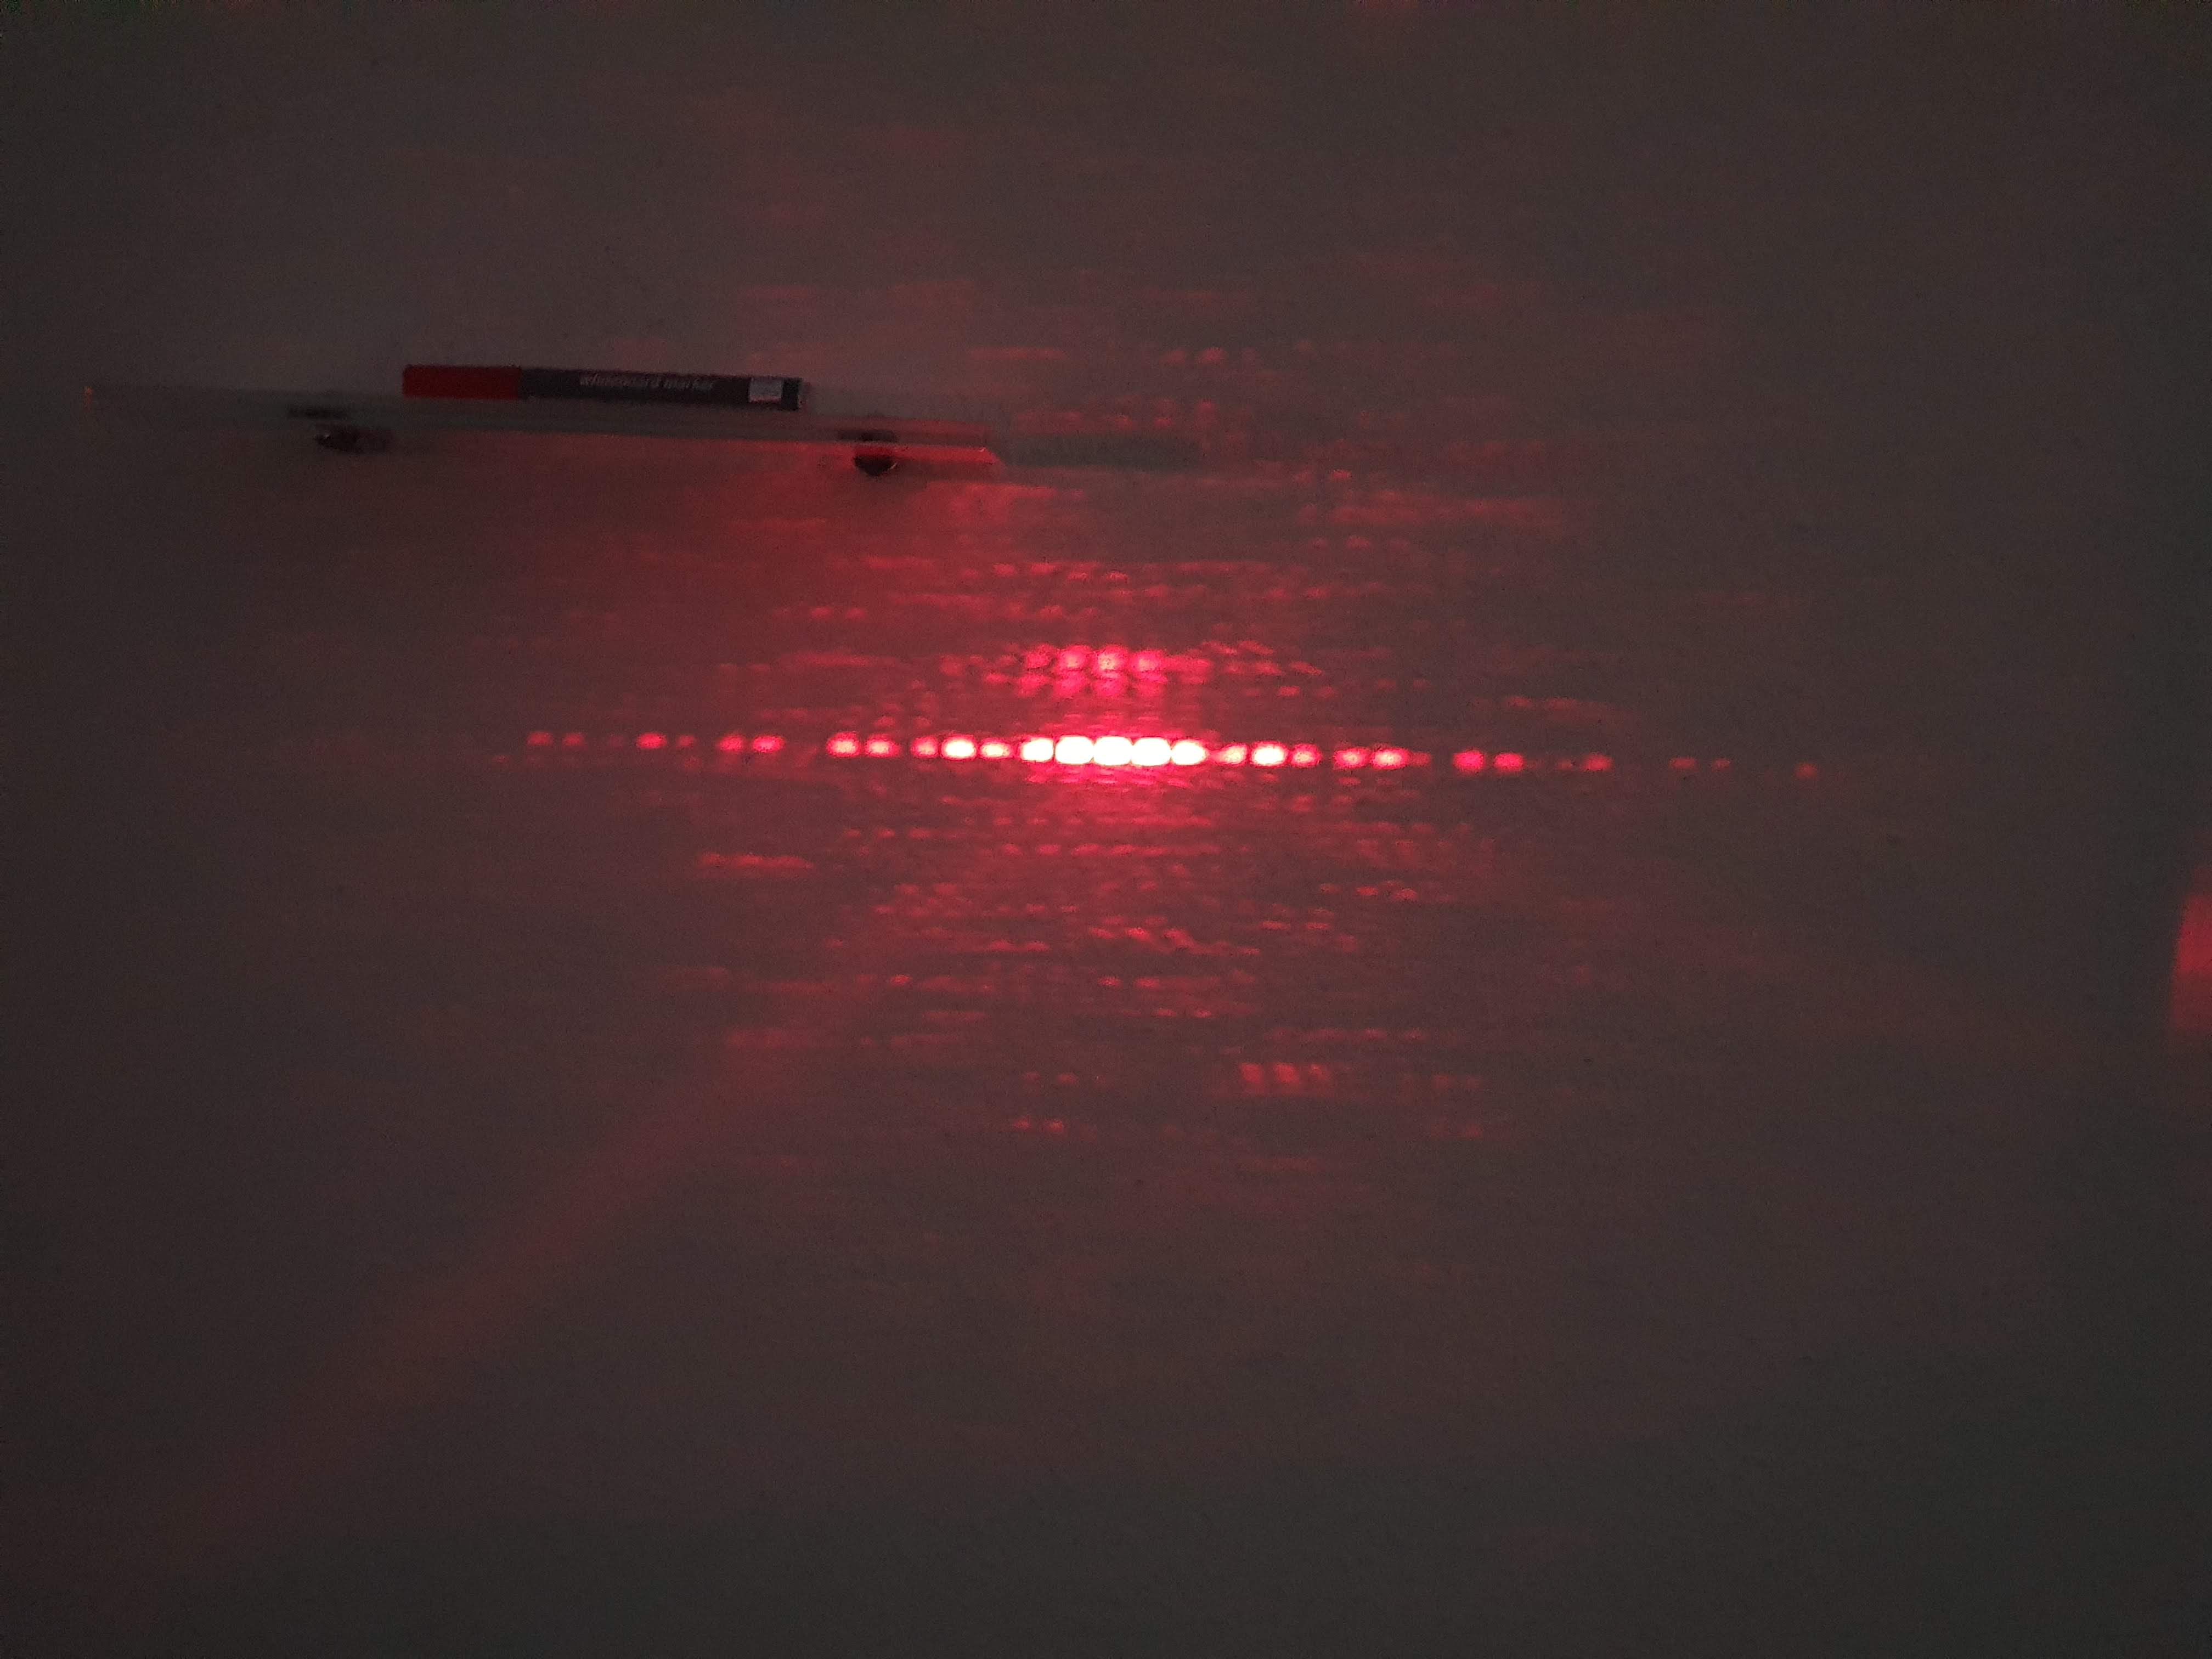
\includegraphics[width=0.22\textwidth]{images/tv5/mehrfachspalt/n_2.jpg} &
					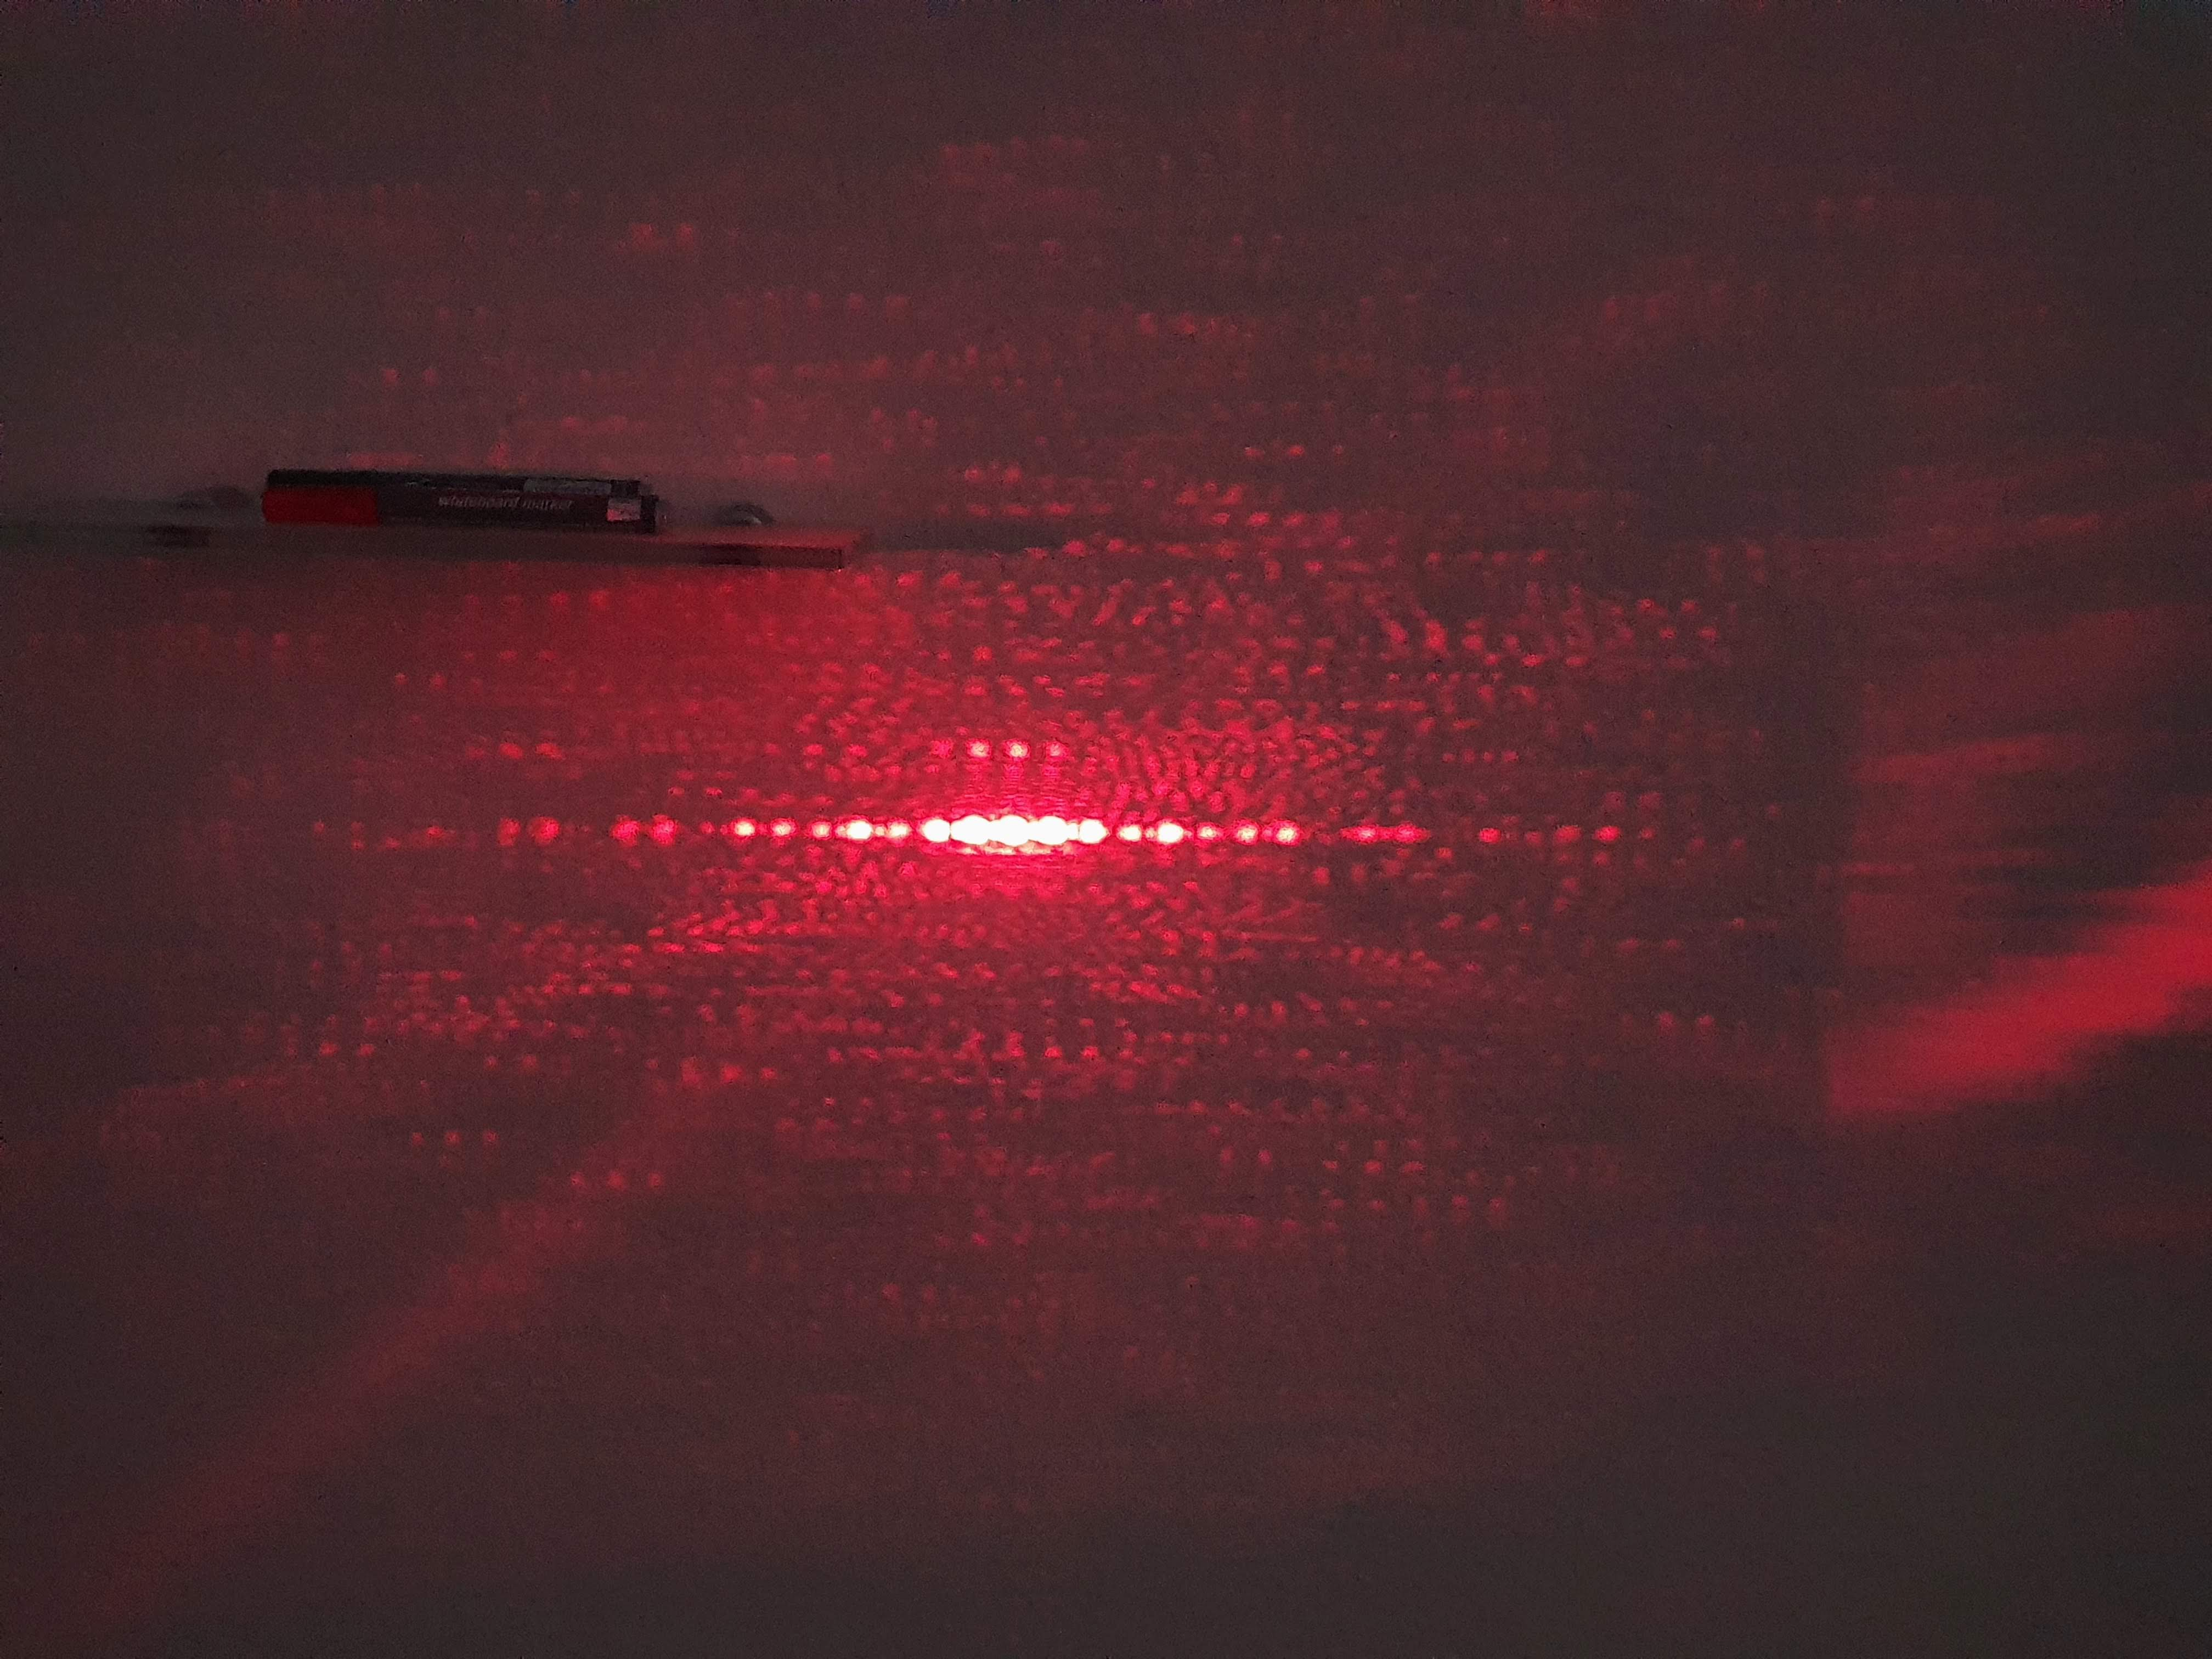
\includegraphics[width=0.22\textwidth]{images/tv5/mehrfachspalt/n_3.jpg} &
					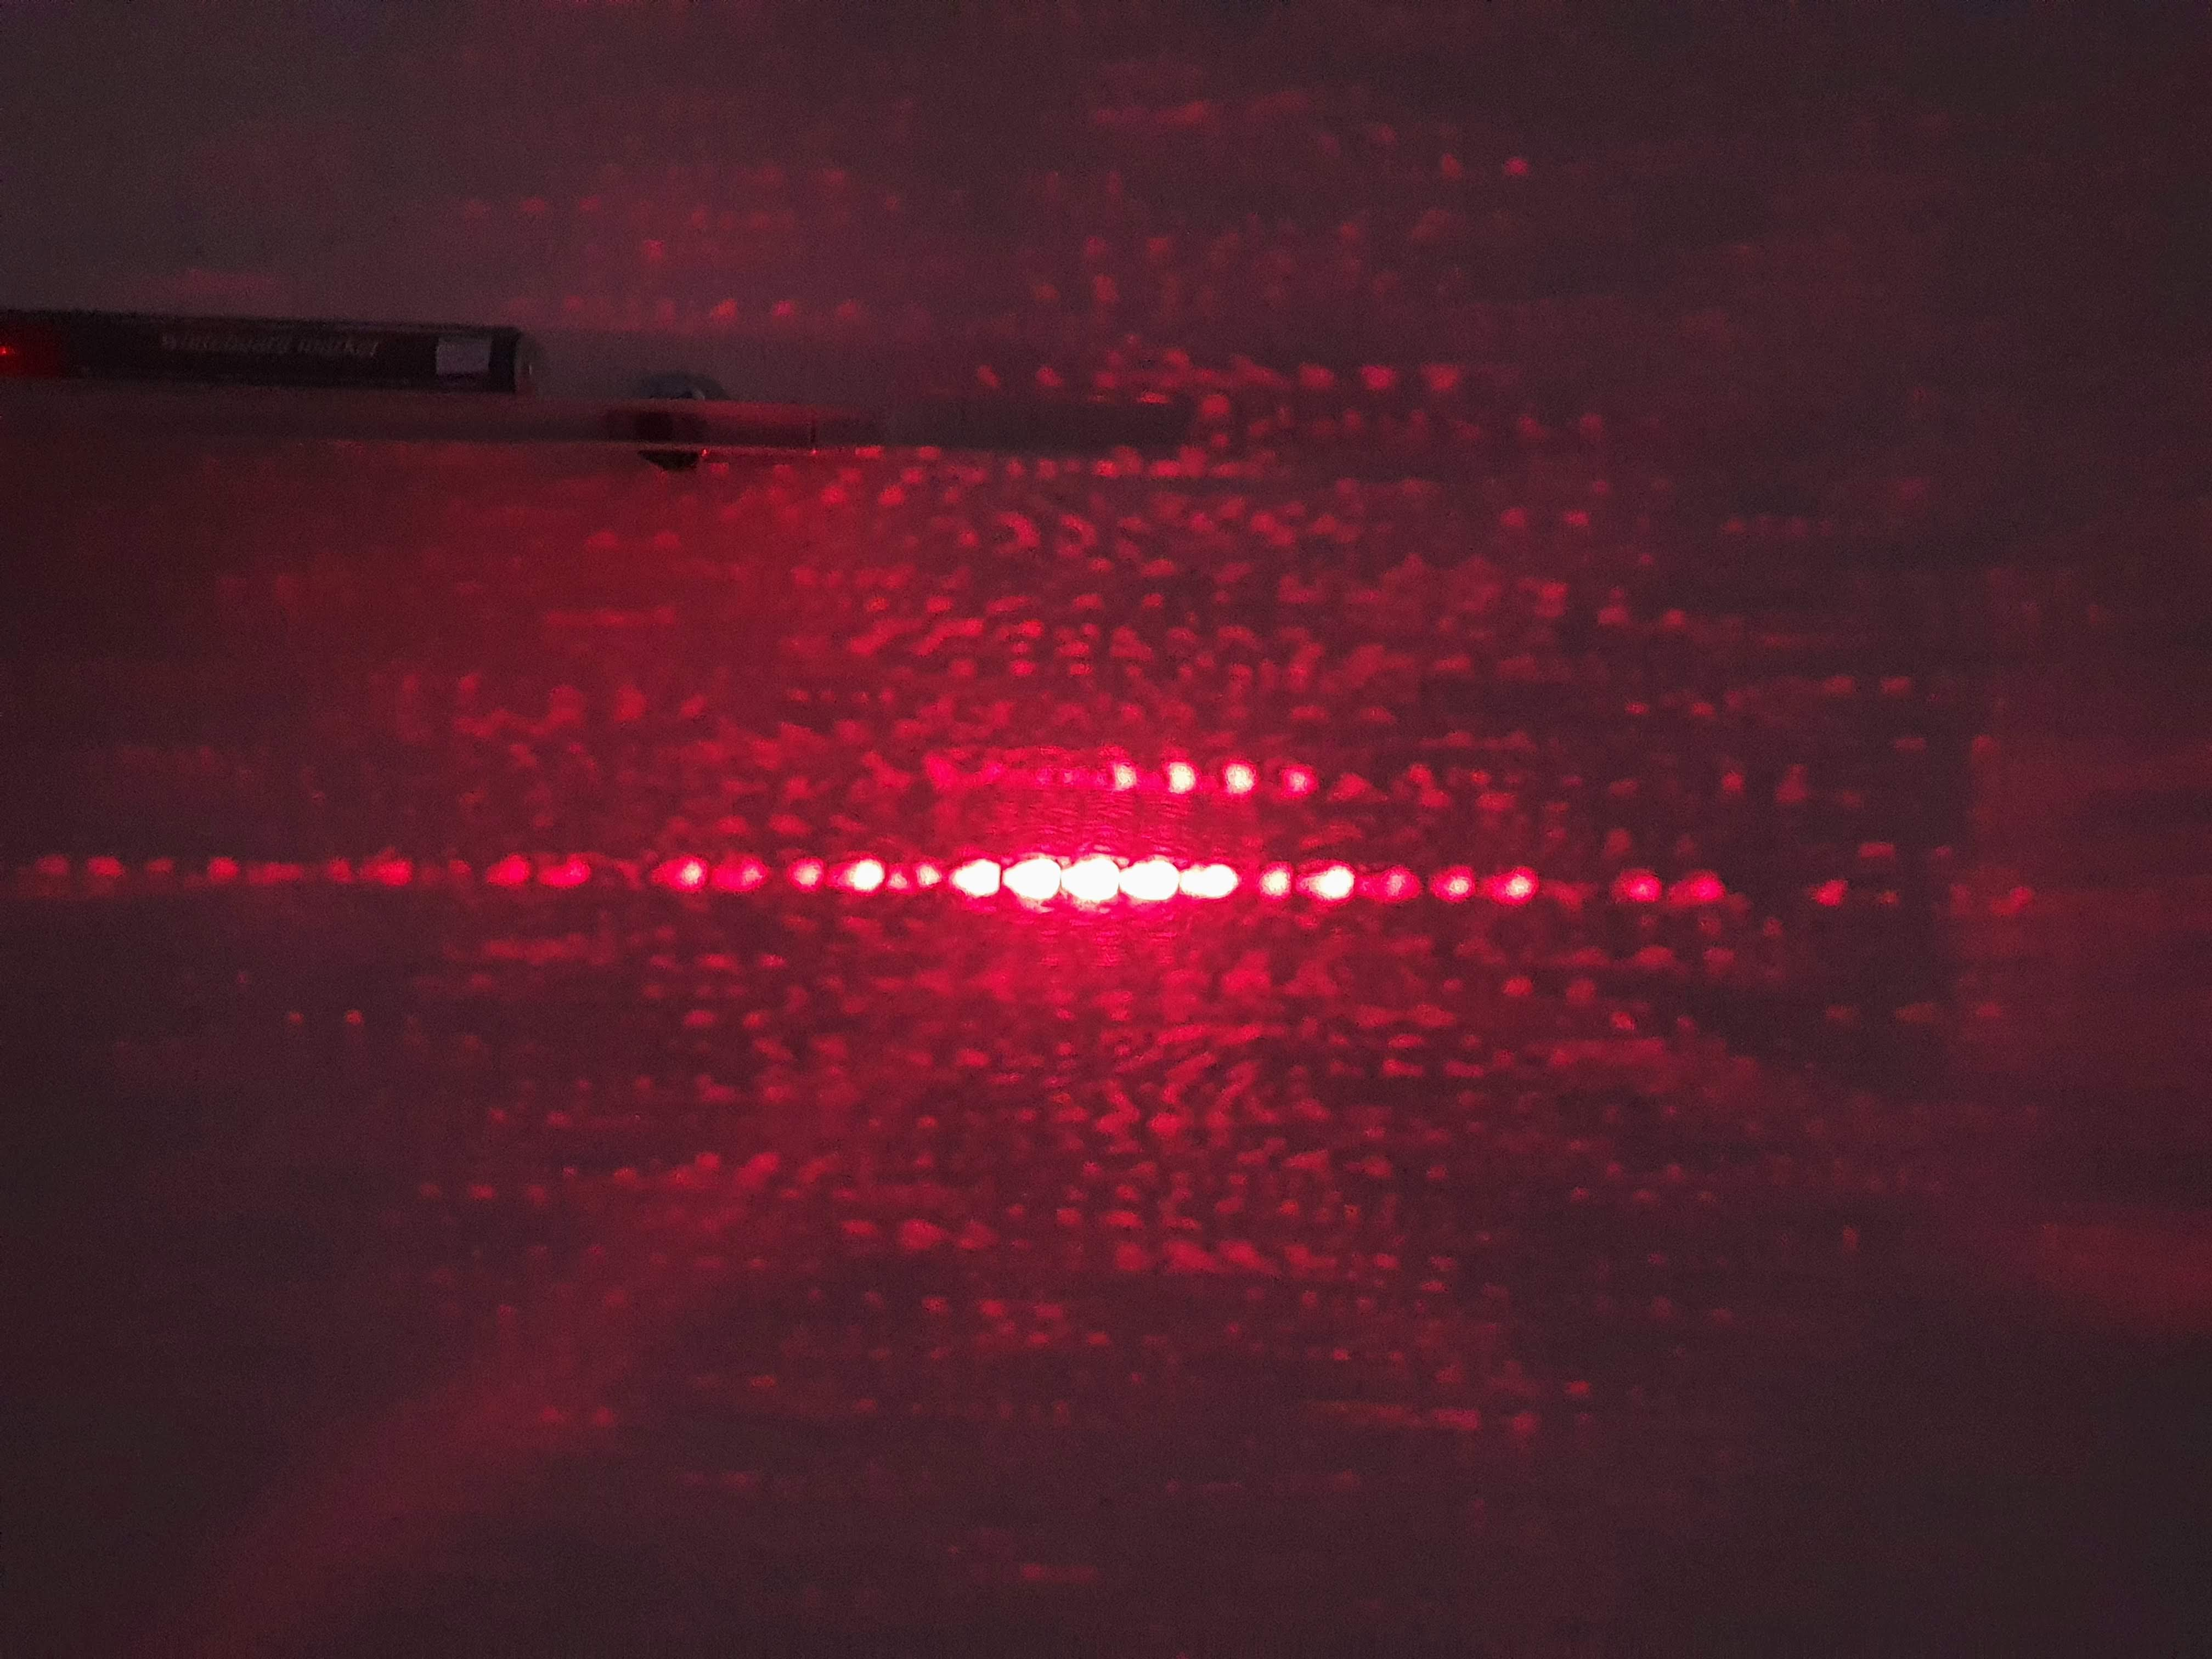
\includegraphics[width=0.22\textwidth]{images/tv5/mehrfachspalt/n_4.jpg} &
					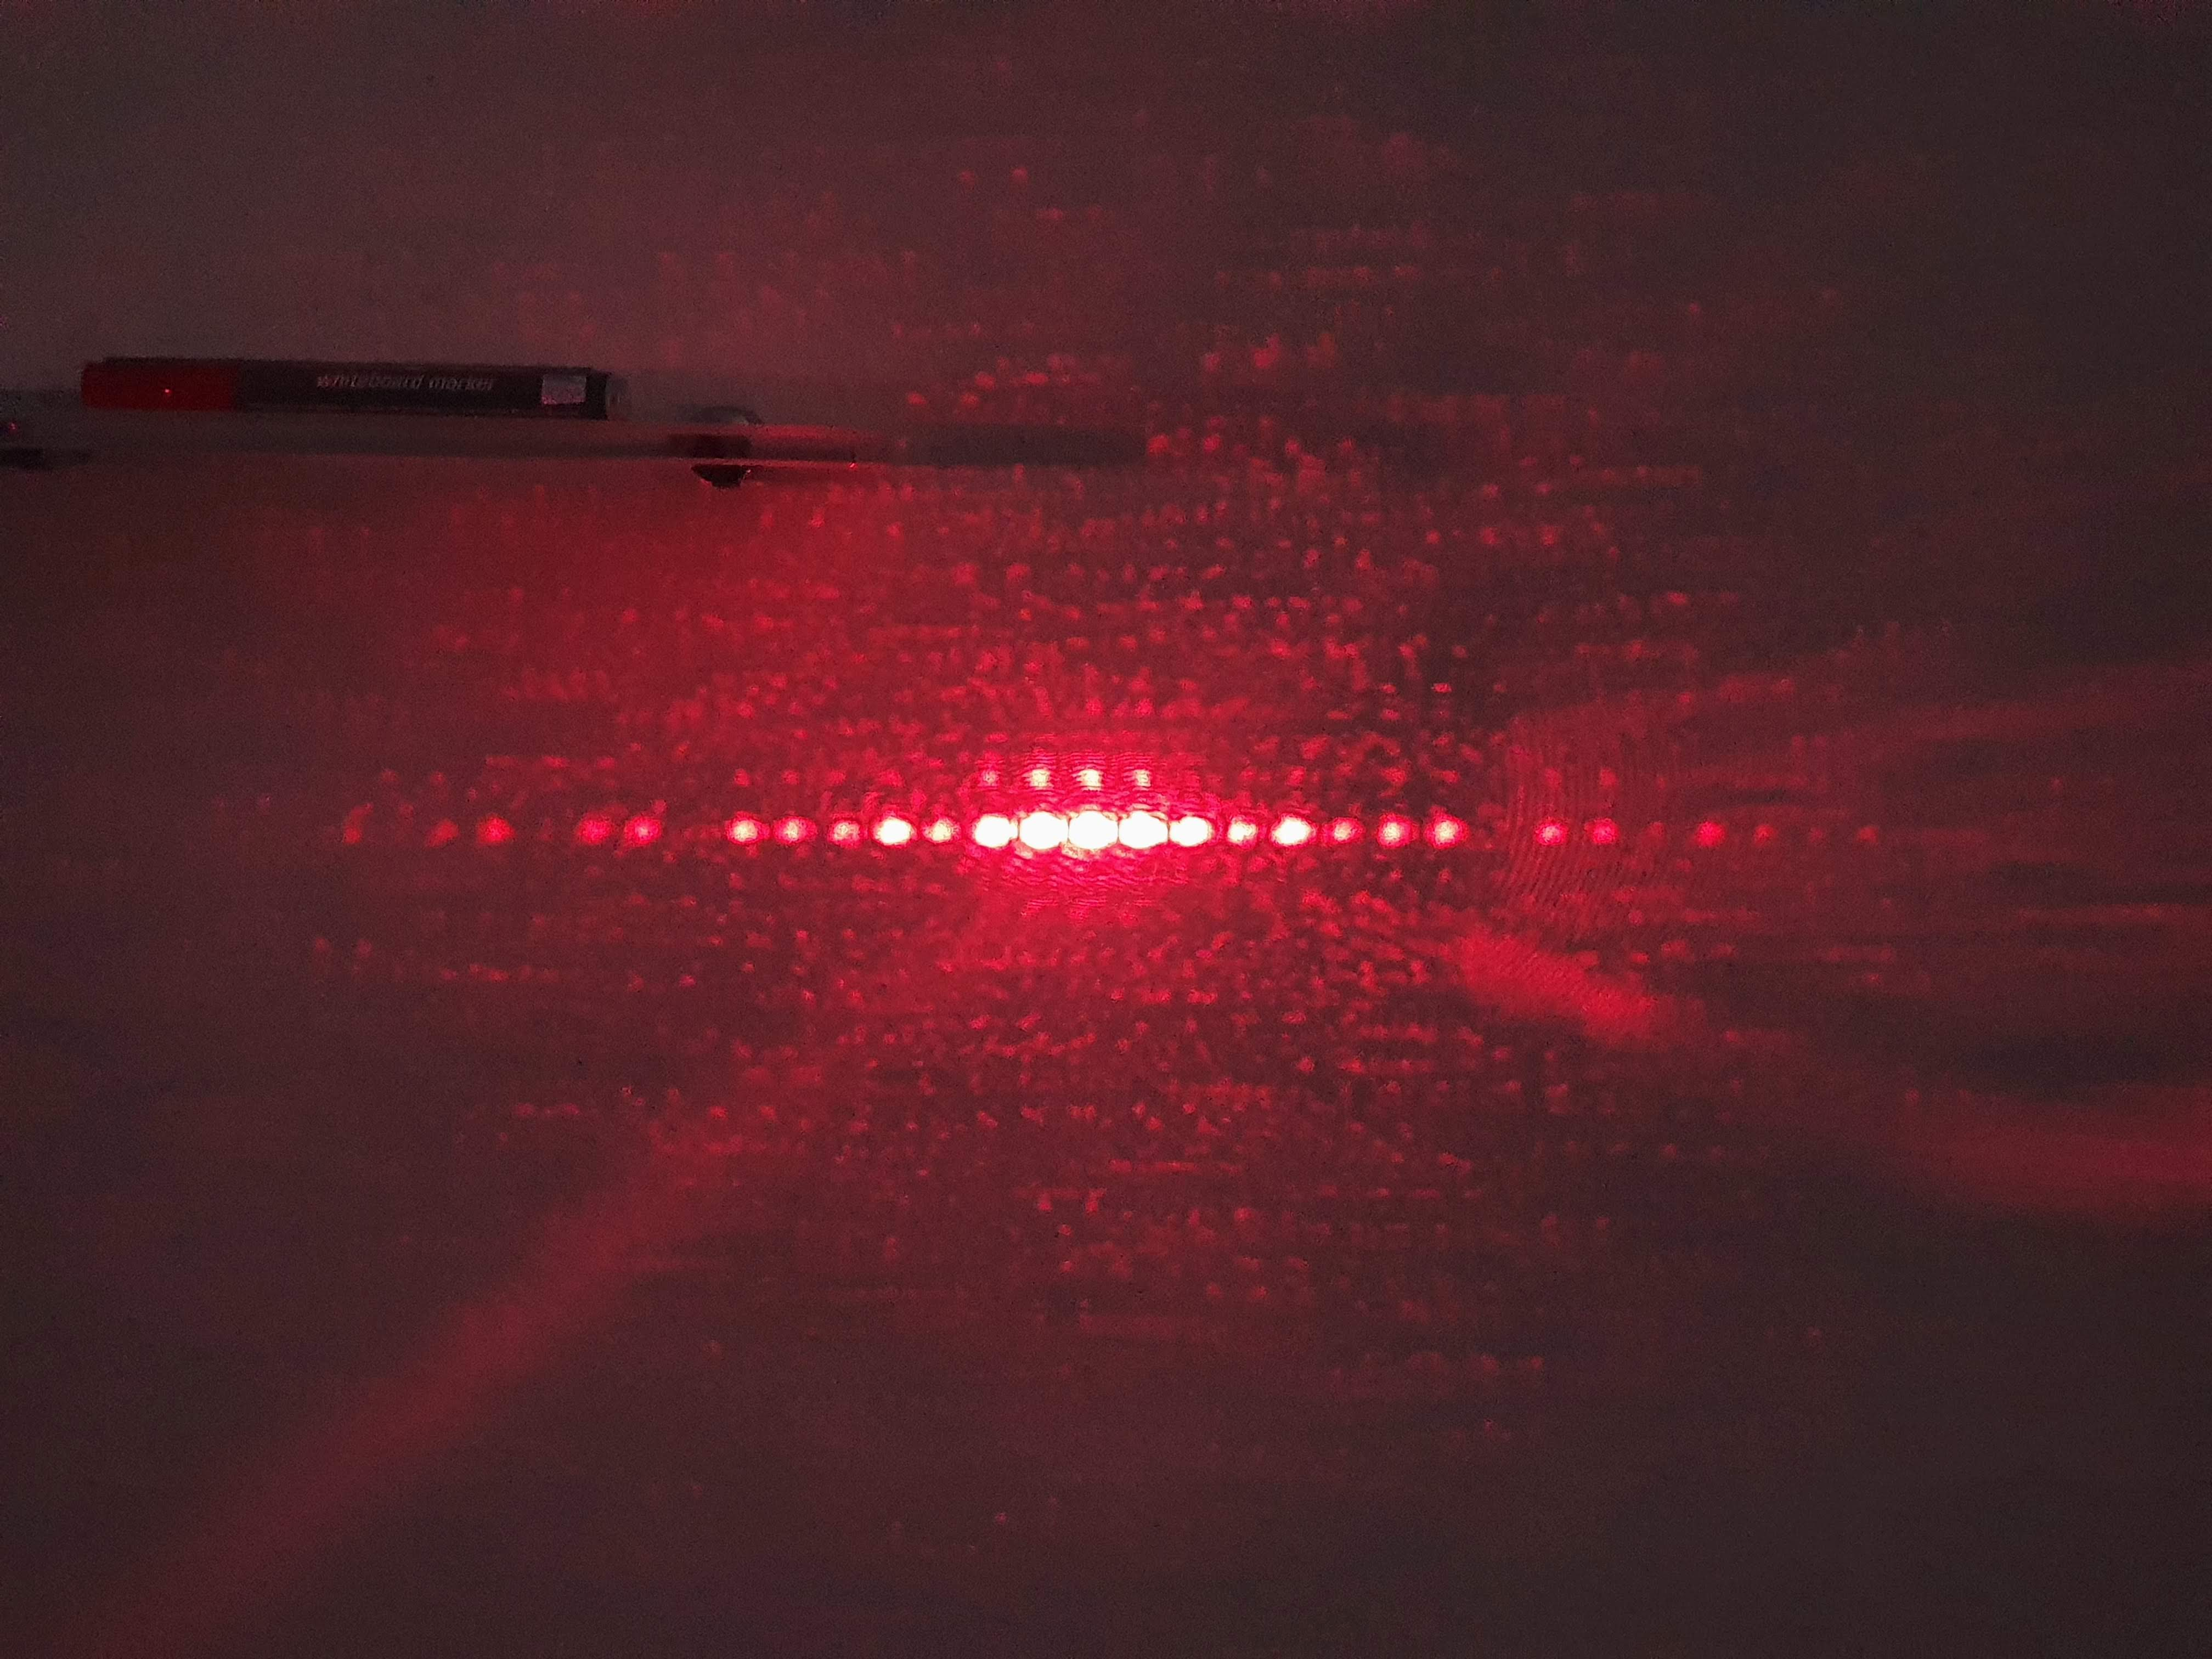
\includegraphics[width=0.22\textwidth]{images/tv5/mehrfachspalt/n_5.jpg} \\
				\bottomrule
			\end{tabular}
		\caption{\centering Beugungsmuster von Doppelspalt und Mehrfachspalt am Wand}
		\vspace{-1em}
		\end{figure}
		Aus der Anleitung gilt die Gleichung:
		\begin{align}
			I(\phi) = 
				\brc{\left(\frac{\sin\left(\frac{\pi b}{\lambda} \sin\phi\right)}{\frac{\pi b}{\lambda} \sin\phi}\right)^2}{\text{Einzelspalt}}
				\brc{\left(\frac{\sin\left(\frac{N\pi g}{\lambda} \sin\phi\right)}{\sin\left(\frac{\pi g}{\lambda} \sin\phi\right)}\right)^2}{\text{Mehrfachspalt}}
		\end{align}
		Es gibt hier zwei Faktoren, die zur Intensität dieses Mustersbeiträgt. Der erste Faktor ist die sinc Funktion, die aus einem Einzelspalt stammt. Die Intensität ist also immer von diese einhüllende Faktor begrenzt. Wir beobachten in allen Beugungsmuster, dass die Intensität abnimmt, je ferner man vom Zentrum ist. Dieser Faktor erklärt dieses Phänomen. Außerdem erkennt man deswegen, dass das einhüllende Intensitätsprofil bei $b = \num{0.2}$ schmaler ist als bei $b = \num{0.1}$, da die Breite dieser Einhüllende direkt vom $b$ abhängt. 

		Im Fall des Doppelspalts gilt:
		\begin{align}
			I(\phi) = 
				\left(\frac{\sin\left(\frac{\pi b}{\lambda} \sin\phi\right)}{\frac{\pi b}{\lambda} \sin\phi}\right)^2
				\left(\frac{\sin\left(\frac{2\pi g}{\lambda} \sin\phi\right)}{\sin\left(\frac{\pi g}{\lambda} \sin\phi\right)}\right)^2
		\end{align}
		Mit dem gleiches $b$ und unterschiedliches $g$ ist nur die 2. Faktor entscheidend und zwar:
		\begin{align}
			I(\phi) \propto
				\left(\frac{\sin\left(\frac{2\pi g}{\lambda} \sin\phi\right)}{\sin\left(\frac{\pi g}{\lambda} \sin\phi\right)}\right)^2
		\end{align}
		Der Paramater $g$ entscheidet also wie breit jede einzelne Maxima ist. Je größer das $g$, desto kleiner das einzelne Maximum ist. Das ist genau was wir bei den rechten 3 Bilder der ersten Reihe erkennen. Bei $g=\num{1,0}$ sind die Maxima so schmal, dass die Kamera wegen die Intensität des Laserstrahls sogar nicht gut unterscheiden konnte. 

		Im Fall des Mehrfachspalts mit gleichen $b$ und $g$ gilt:
		\begin{align}
			I(\phi) \propto
				\left(\frac{\sin\left(\frac{N\pi g}{\lambda} \sin\phi\right)}{\sin\left(\frac{\pi g}{\lambda} \sin\phi\right)}\right)^2
		\end{align}
		Der Parameter $N$ entscheidet wiederum wie breit jede einzelne Maxima ist, aber da es nur im Zähler steht, ist das Effekt deutlich kleiner. was auch im Versuch zu beobachten ist. 

